\subsection{Symbolic Execution}

\subsubsection{Simple Computation}

\descriptionproblem
Consider the following fragment of code:
\lstinputlisting[language=C, firstnumber=0]{code/symbolic-execution-1.c}

\questionproblem
\begin{enumerate}
    \item Derive the path condition corresponding to the execution of path:
    \begin{equation*}
        < 1, 2, 4, 5, 6, 7, 8, 10, 11, 12, 7, 8, 9, 10, 11, 12, 7, 13, 14 >
    \end{equation*}
    
    \item Derive the path condition corresponding to the execution of path:
    \begin{equation*}
        < 1, 2, 4, 5, 6, 7, 13, 15 >
    \end{equation*}
\end{enumerate}

\solution
The symbolic execution analyses a program to determine what inputs cause each part of a program to execute. The full explanation can be found in section~\ref{subsection: Analysis - Symbolic Execution} on page~\pageref{subsection: Analysis - Symbolic Execution}.

\highspace
The answer to both questions:
\begin{itemize}
    \item Path: $0$
    \begin{figure}[!htp]
        \centering
        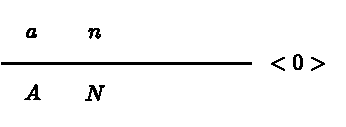
\includegraphics[width=.5\textwidth]{img/symbolic-execution-1.pdf}
    \end{figure}

    \newpage

    \item Path: $0, 1$
    \begin{figure}[!htp]
        \centering
        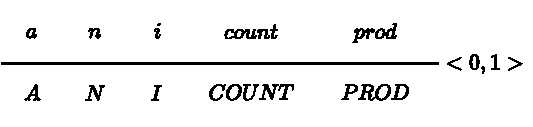
\includegraphics[width=.7\textwidth]{img/symbolic-execution-2.pdf}
    \end{figure}

    \item Path: $0, 1, 2$
    \begin{figure}[!htp]
        \centering
        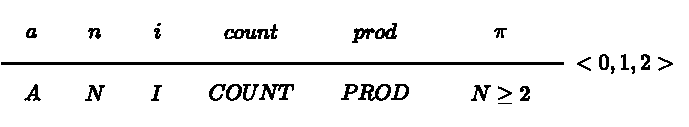
\includegraphics[width=.7\textwidth]{img/symbolic-execution-3.pdf}
    \end{figure}

    \item Path: $0, 1, 2, 4$
    \begin{figure}[!htp]
        \centering
        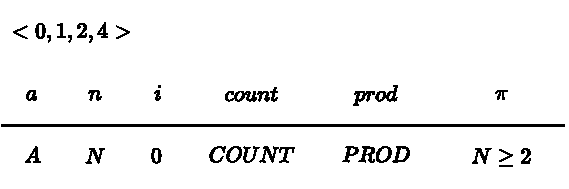
\includegraphics[width=.7\textwidth]{img/symbolic-execution-4.pdf}
    \end{figure}

    \item Path: $0, 1, 2, 4, 5, 6$
    \begin{figure}[!htp]
        \centering
        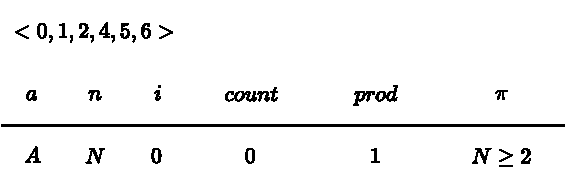
\includegraphics[width=.7\textwidth]{img/symbolic-execution-5.pdf}
    \end{figure}
\end{itemize}

\newpage

\noindent
Here is the answer to the first question (\textbf{\underline{solution 1}}):
\begin{itemize}
    \item Path: $0, 1, 2, 4, 5, 6, 7$
    \begin{figure}[!htp]
        \centering
        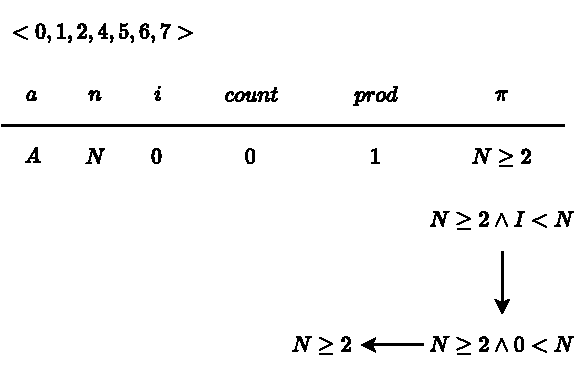
\includegraphics[width=.7\textwidth]{img/symbolic-execution-6.pdf}
    \end{figure}

    \item Path: $0, 1, 2, 4, 5, 6, 7, 8$
    \begin{figure}[!htp]
        \centering
        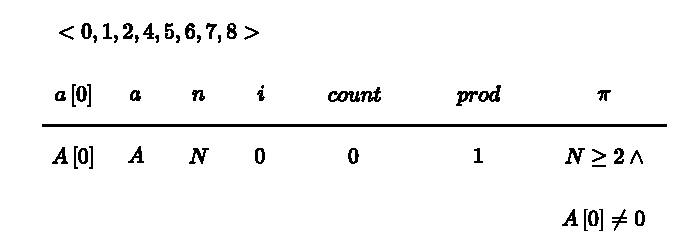
\includegraphics[width=.8\textwidth]{img/symbolic-execution-7.pdf}
    \end{figure}

    \item Path: $0, 1, 2, 4, 5, 6, 7, 8, 10$
    \begin{figure}[!htp]
        \centering
        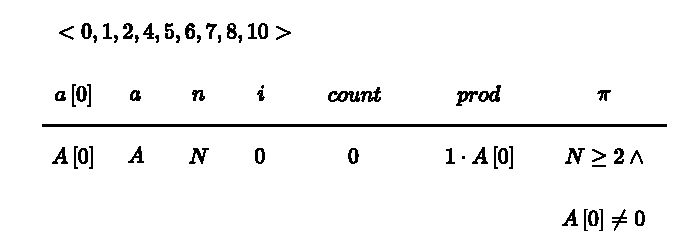
\includegraphics[width=.8\textwidth]{img/symbolic-execution-8.pdf}
    \end{figure}

    \newpage

    \item Path: $0, 1, 2, 4, 5, 6, 7, 8, 10, 11, 12$
    \begin{figure}[!htp]
        \centering
        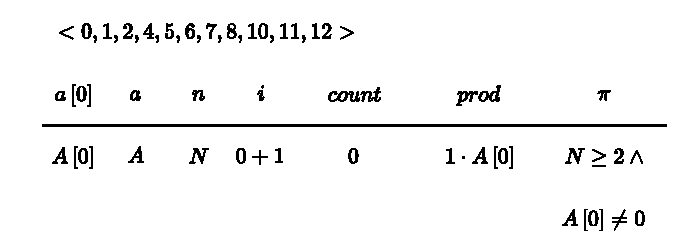
\includegraphics[width=.8\textwidth]{img/symbolic-execution-9.pdf}
    \end{figure}

    \item Path: $0, 1, 2, 4, 5, 6, 7, 8, 10, 11, 12, 7$
    \begin{figure}[!htp]
        \centering
        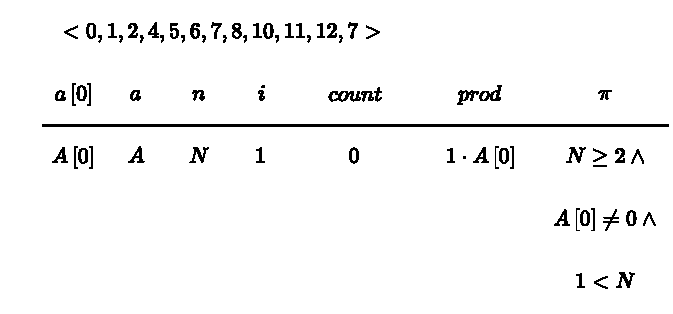
\includegraphics[width=.8\textwidth]{img/symbolic-execution-10.pdf}
    \end{figure}

    \item Path: $0, 1, 2, 4, 5, 6, 7, 8, 10, 11, 12, 7, 8, 9$
    \begin{figure}[!htp]
        \centering
        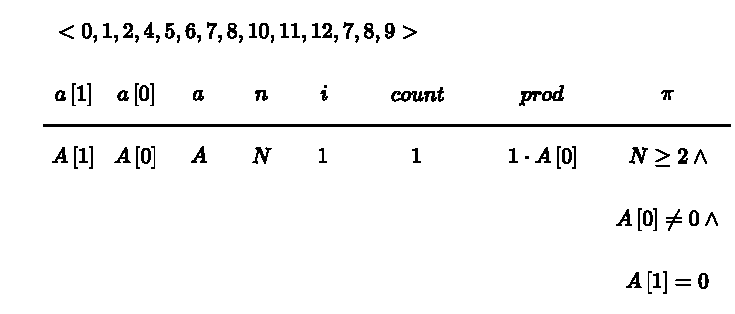
\includegraphics[width=.8\textwidth]{img/symbolic-execution-11.pdf}
    \end{figure}

    \newpage

    \item Path: $0, 1, 2, 4, 5, 6, 7, 8, 10, 11, 12, 7, 8, 9, 10$
    \begin{figure}[!htp]
        \centering
        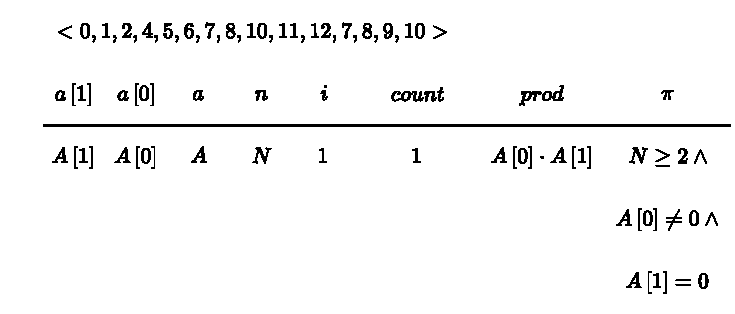
\includegraphics[width=.8\textwidth]{img/symbolic-execution-12.pdf}
    \end{figure}

    \item Path: $0, 1, 2, 4, 5, 6, 7, 8, 10, 11, 12, 7, 8, 9, 10, 11, 12$
    \begin{figure}[!htp]
        \centering
        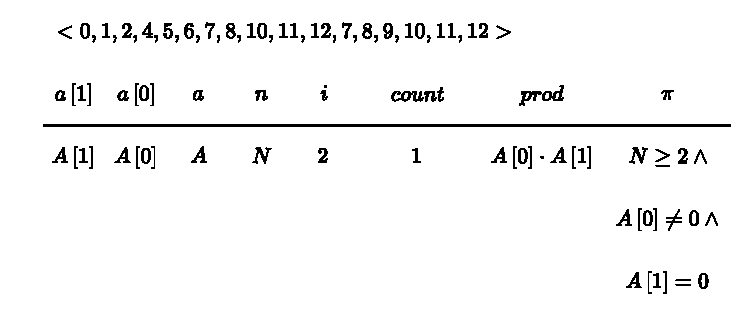
\includegraphics[width=.8\textwidth]{img/symbolic-execution-13.pdf}
    \end{figure}

    \item Path: $0, 1, 2, 4, 5, 6, 7, 8, 10, 11, 12, 7, 8, 9, 10, 11, 12, 7$
    \begin{figure}[!htp]
        \centering
        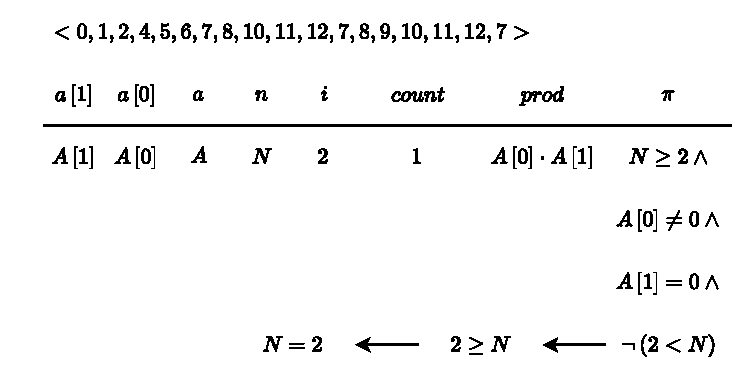
\includegraphics[width=.8\textwidth]{img/symbolic-execution-14.pdf}
    \end{figure}

    \newpage

    \item Path: $0, 1, 2, 4, 5, 6, 7, 8, 10, 11, 12, 7, 8, 9, 10, 11, 12, 7, 13, 14$
    \begin{figure}[!htp]
        \centering
        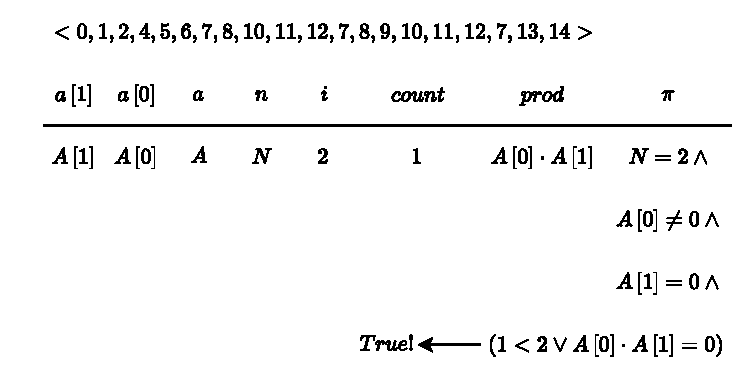
\includegraphics[width=.8\textwidth]{img/symbolic-execution-15.pdf}
    \end{figure}
\end{itemize}
This path is \emph{satisfiable}. An unsatisfiable case is \textbf{\underline{solution}} number \textbf{\underline{2}}:
\begin{itemize}
    \item Path: $0, 1, 2, 4, 5, 6, 7$
    \begin{figure}[!htp]
        \centering
        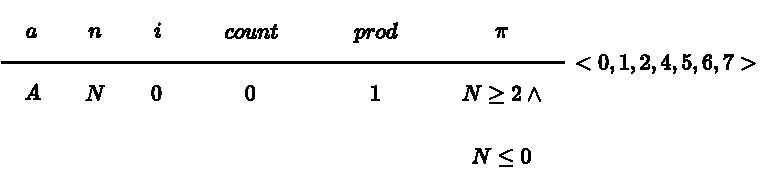
\includegraphics[width=\textwidth]{img/symbolic-execution-16.pdf}
    \end{figure}
\end{itemize}
It's unsatisfiable because the logical condition is a contradiction: $N \ge 2 \land N \le 0$.